\addsec{Anhang}

\subsection*{Anlage 1}
\label{subsec: Anlage1}

\textbf{Allgemeine Grenzwerte zu Blitzen und roten Blitzen (general flash and red flash thresholds)}\footnote{Web Content Accessibility Guidelines 2.0 \cite{WCAG2.0}}

\begin{enumerate}
	\item Ein Blitz oder eine schnell wechselnde Sequenz von Bildern ist unterhalb des Grenzwertes (d.h. Inhalt besteht die Prüfung), wenn eines der Folgenden zutrifft:
	Es gibt nicht mehr als drei allgemeine Blitze und / oder nicht mehr als drei rote Blitze innerhalb von beliebigen Ein-Sekunden-Zeiträumen; oder

	\item Der zusammengenommene Bereich von gleichzeitig auftretenden Blitzen belegt nicht mehr als eine Summe von .006 Steradianten innerhalb jedes beliebigen 10 Grad 		visuellen Feldes auf dem Bildschirm (25\% jedes beliebigen 10-Grad visuellen Feldes auf dem Bildschirm) bei einer typischen Betrachtungsentfernung. Wobei:
	\begin{itemize}
		\item Ein allgemeiner Blitz als ein Paar von entgegengesetzten Änderungen in relativer Luminanz von 10\% oder mehr der maximalen relativen Luminanz definiert wird, 		wobei die relative Luminanz des dunkleren Bildes unter 0.80 liegt; und wo „ein Paar von entgegengesetzten Änderungen“ eine Zunahme gefolgt von einer Abnahme 				ist oder eine Abnahme gefolgt von einer Zunahme. Und
		\item Ein roter Blitz als jedes Paar von entgegengesetzten Übergängen, bei denen ein gesättigtes Rot beteiligt ist, definiert wird.
	\end{itemize}
\end{enumerate}

\textbf{Ausnahme:} Blitzen, das ein feines, ausgeglichenes Muster wie weißes Rauschen oder ein wechselndes Schachbrettmuster mit "`Quadraten"' ist, die auf einer Seite kleiner sind als 0.1 Grad (des visuellen Feldes bei typischem Betrachtungsabstand), verstößt nicht gegen die Grenzwerte.

\textbf{Anmerkung 1:} Die Benutzung eines 341 x 256 Pixel großen Rechtecks irgendwo in dem gezeigten Bildschirmbereich, wenn der Inhalt bei 1024 x 768 Pixeln betrachtet wird, gibt bei allgemeiner Software oder Webinhalten eine gute Einschätzung eines 10 Grad visuellen Feldes für Standard-Bildschirmgrößen und Betrachtungsentfernungen (z.B. 15-17 Zoll Bildschirm bei 56 - 66 cm). (Bildschirme mit höheren Auflösungen, auf denen das gleiche Rendering des Inhalts gezeigt wird, ergeben kleinere und sicherere Bilder, daher werden die geringeren Auflösungen benutzt, um die Grenzwerte zu definieren.)

\textbf{Anmerkung 2:} Ein Übergang ist der Wechsel in relativer Luminanz (oder relativer Luminanz/Farbe für rotes Blitzen) zwischen nebeneinander liegenden Spitzen und Senken in einem Graph von relativer Luminanzmessung (oder relativer Luminanz/Farbe bei rotem Blitzen) in Bezug auf die Zeit. Ein Blitz besteht aus zwei entgegengesetzten Änderungen.

\textbf{Anmerkung 3:} Die derzeitige Arbeitsdefinition in diesem Fachbereich für ein "`Paar von entgegengesetzten Übergängen, die ein gesättigtes Rot beinhalten"' lautet: Wenn für jeden oder beide Zustände, die in jedem Übergang involviert sind, R/(R+ G + B) >= 0.8 und der Wechsel des Wertes von (R-G-B)x320 > 20 (negative Werte von (R-G-B)x320 werden auf Null gesetzt) für beide Übergänge ist. R, G, B Werte reichen von 0-1 wie in der "`relativen Luminanz"'-Definition festgelegt. [HARDING-BINNIE]

\textbf{Anmerkung 4:} Es gibt Werkzeuge, welche die Analyse durch die Erfassung des Video-Bildschirms ausführen. Es ist allerdings kein Werkzeug nötig, um diese Bedingung zu evaluieren, wenn das Blitzen weniger oder gleich 3 Blitze pro Sekunde ist. Der Inhalt besteht automatisch die Prüfung (siehe \# 1 und \# 2 oben).

\appendix

\subsection*{Anlage 2}
\label{subsec: Anlage2}

\textbf{Input Purposes for User Interface Components}


\noindent This section contains a listing of common user interface component input purposes. The terms below are not keywords that must be used, but instead represent purposes that must be captured in the taxonomy adopted by a webpage. Where applicable, authors mark up controls with the chosen taxonomy to indicate the semantic purpose. This provides the potential for user agents and assistive technologies to apply personalized presentations that can enable more people to understand and use the content.\\

\noindent \textit{NOTE}
The list of input type purposes is based on the control purposes defined in the HTML 5.2 Autofill field section, but it is important to understand that a different technology may have some or all of the same concepts defined in its specification and only the concepts that are mapped to the meanings below are required.\\

\noindent The following input control purposes are intended to relate to the user of the content and pertain only to information related to that individual.
\begin{itemize}
\item name - Full name
\item honorific-prefix - Prefix or title (e.g., "Mr.", "Ms.", "Dr.", "Mlle")
\item given-name - Given name (in some Western cultures, also known as the first name)
\item additional-name - Additional names (in some Western cultures, also known as middle names, forenames other than the first name)
\item family-name - Family name (in some Western cultures, also known as the last name or surname)
\item honorific-suffix - Suffix (e.g., "Jr.", "B.Sc.", "MBASW", "II")
\item nickname - Nickname, screen name, handle: a typically short name used instead of the full name
\item organization-title - Job title (e.g., "Software Engineer", "Senior Vice President", "Deputy Managing Director")
\item username - A username
\item new-password - A new password (e.g., when creating an account or changing a password)
\item current-password - The current password for the account identified by the username field (e.g., when logging in)
\item organization - Company name corresponding to the person, address, or contact information in the other fields associated with this field
\item street-address - Street address (multiple lines, newlines preserved)
\item address-line1 - Street address (one line per field, line 1)
\item address-line2 - Street address (one line per field, line 2)
\item address-line3 - Street address (one line per field, line 3)
\item address-level4 - The most fine-grained administrative level, in addresses with four administrative levels
\item address-level3 - The third administrative level, in addresses with three or more administrative levels
\item address-level2 - The second administrative level, in addresses with two or more administrative levels; in the countries with two administrative levels, this would typically be the city, town, village, or other locality within which the relevant street address is found
\item address-level1 - The broadest administrative level in the address, i.e., the province within which the locality is found; for example, in the US, this would be the state; in Switzerland it would be the canton; in the UK, the post town
\item country - Country code
\item country-name - Country name
\item postal-code - Postal code, post code, ZIP code, CEDEX code (if CEDEX, append "CEDEX", and the dissement, if relevant, to the address-level2 field)
\item cc-name - Full name as given on the payment instrument
\item cc-given-name - Given name as given on the payment instrument (in some Western cultures, also known as the first name)
\item cc-additional-name - Additional names given on the payment instrument (in some Western cultures, also known as middle names, forenames other than the first name)
\item cc-family-name - Family name given on the payment instrument (in some Western cultures, also known as the last name or surname)
\item cc-number - Code identifying the payment instrument (e.g., the credit card number)
\item cc-exp - Expiration date of the payment instrument
\item cc-exp-month - Month component of the expiration date of the payment instrument
\item cc-exp-year - Year component of the expiration date of the payment instrument
\item cc-csc - Security code for the payment instrument (also known as the card security code (CSC), card validation code (CVC), card verification value (CVV), signature panel code (SPC), credit card ID (CCID), etc)
\item cc-type - Type of payment instrument
\item transaction-currency - The currency that the user would prefer the transaction to use
\item transaction-amount - The amount that the user would like for the transaction (e.g., when entering a bid or sale price)
\item language - Preferred language
\item bday - Birthday
\item bday-day - Day component of birthday
\item bday-month - Month component of birthday
\item bday-year - Year component of birthday
\item sex - Gender identity (e.g., Female, Fa’afafine)
\item url - Home page or other Web page corresponding to the company, person, address, or contact information in the other fields associated with this field
\item photo - Photograph, icon, or other image corresponding to the company, person, address, or contact information in the other fields associated with this field
\item tel - Full telephone number, including country code
\item tel-country-code - Country code component of the telephone number
\item tel-national - Telephone number without the county code component, with a country-internal prefix applied if applicable
\item tel-area-code - Area code component of the telephone number, with a country-internal prefix applied if applicable
\item tel-local - Telephone number without the country code and area code components
\item tel-local-prefix - First part of the component of the telephone number that follows the area code, when that component is split into two components
\item tel-local-suffix - Second part of the component of the telephone number that follows the area code, when that component is split into two components
\item tel-extension - Telephone number internal extension code
\item email - E-mail address
\item impp - URL representing an instant messaging protocol endpoint (for example, "aim:goim?screenname=example" or "xmpp:fred@example.net")
\end{itemize}

\subsection*{Anlage 3}
\label{subsec: Anlage3}

\textbf{Wesentliche Unterschiede zwischen Web- und Desktopanwendungen}\footnote{Eigene Darstellung}

\addcontentsline{lot}{table}{1 \hspace{1.5em} Wesentliche Unterschiede zwischen  Web- und Desktopanwendungen}
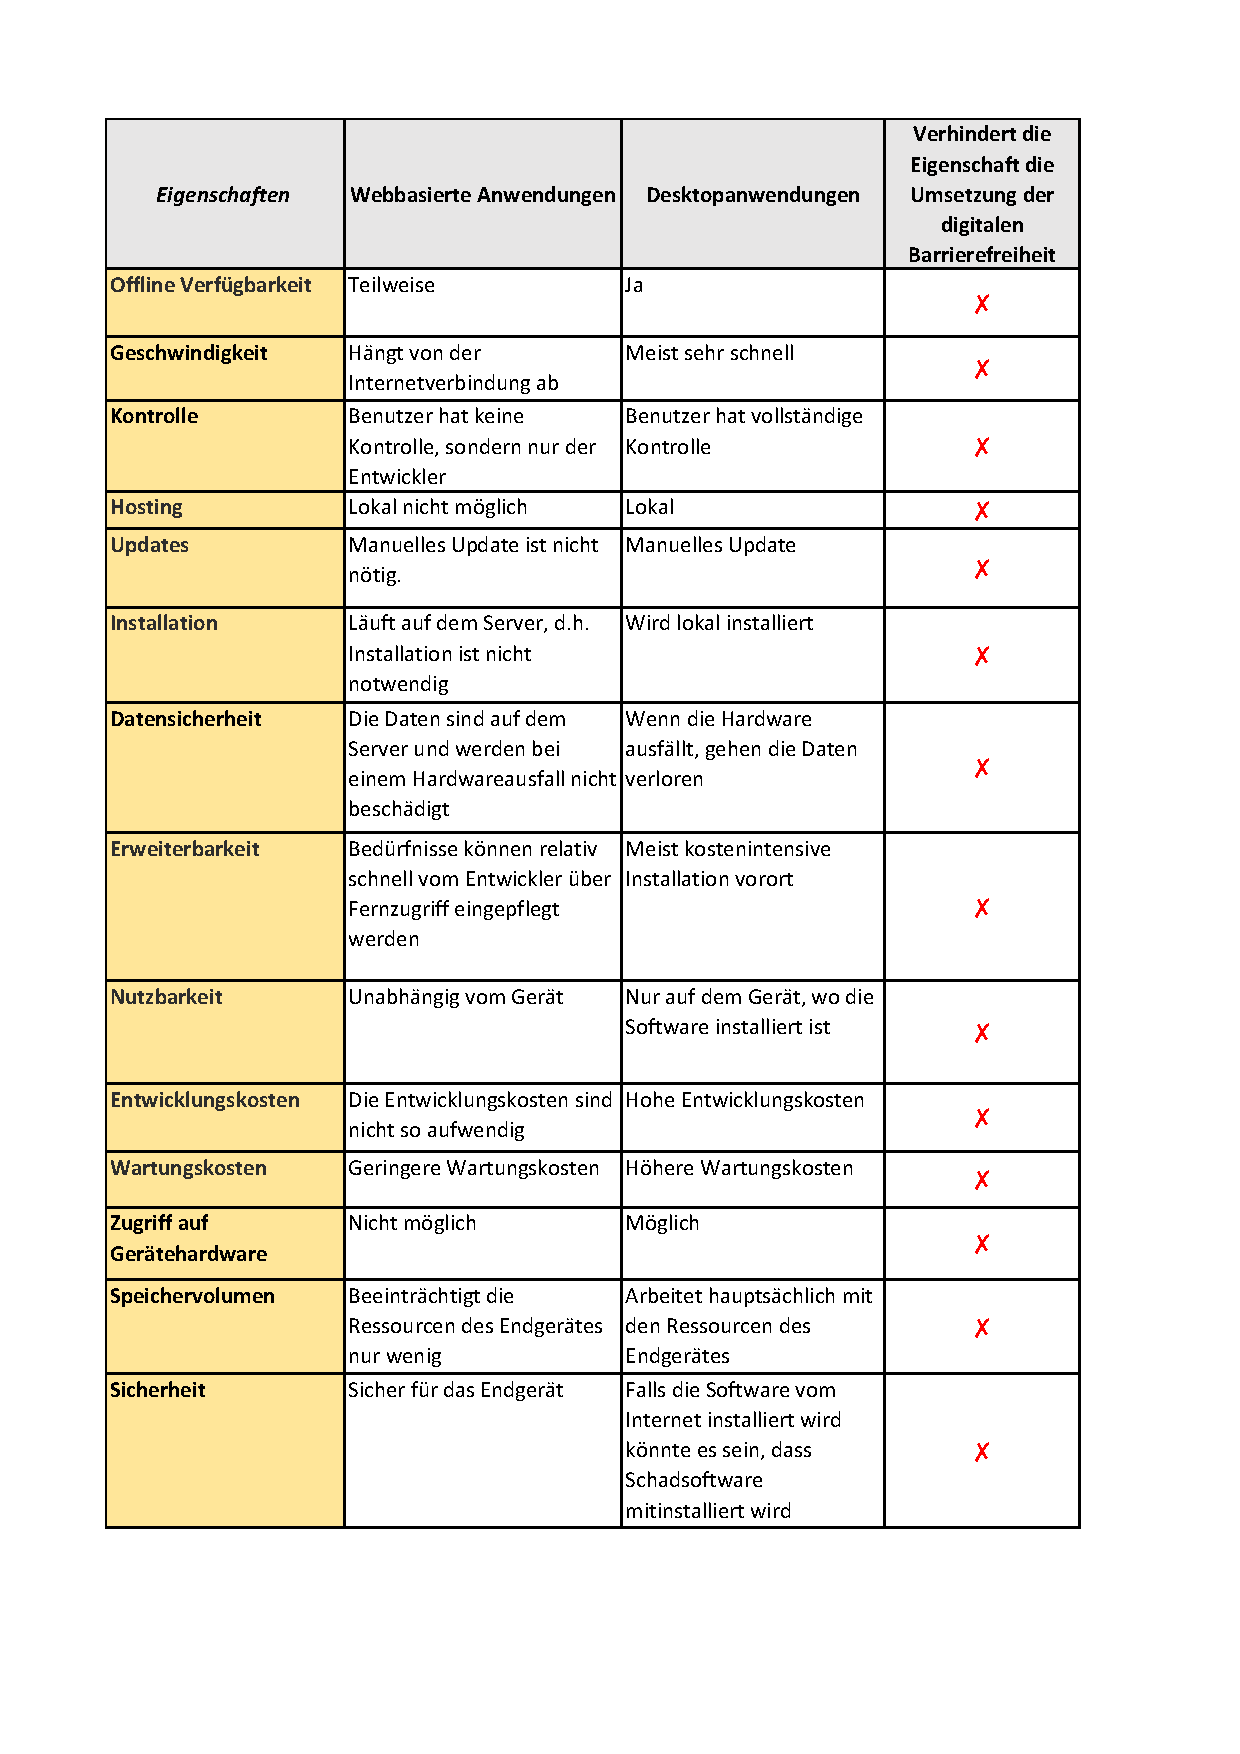
\includepdf[pages=-, scale=0.9, pagecommand={}]{Webanwendungen vs Desktopanwendung}

\subsection*{Anlage 4}
\label{subsec: Anlage4}

\begin{description}
	\item[Text-Kontras Minimum] \hfill \\
	Das Minimum des Kontrastverhältnises von der Textfarbe zur Hintergrundfarbe liegt bei 4,5:1 (3 zu 1) für den normalen Text (kleiner als 14pt) und für größer als 14pt liegt das Minimum bei 3:1. 
	Das Text-Kontrastverhältnis vom Dialog in \cref{fig: Text-Kontrast} wurde durch Eingabe der RGB-Werte der Text- und Hintergrundfarbe in einem Online-Kontrasttester getestet.
	
	\begin{figure}[H]
		\centering
		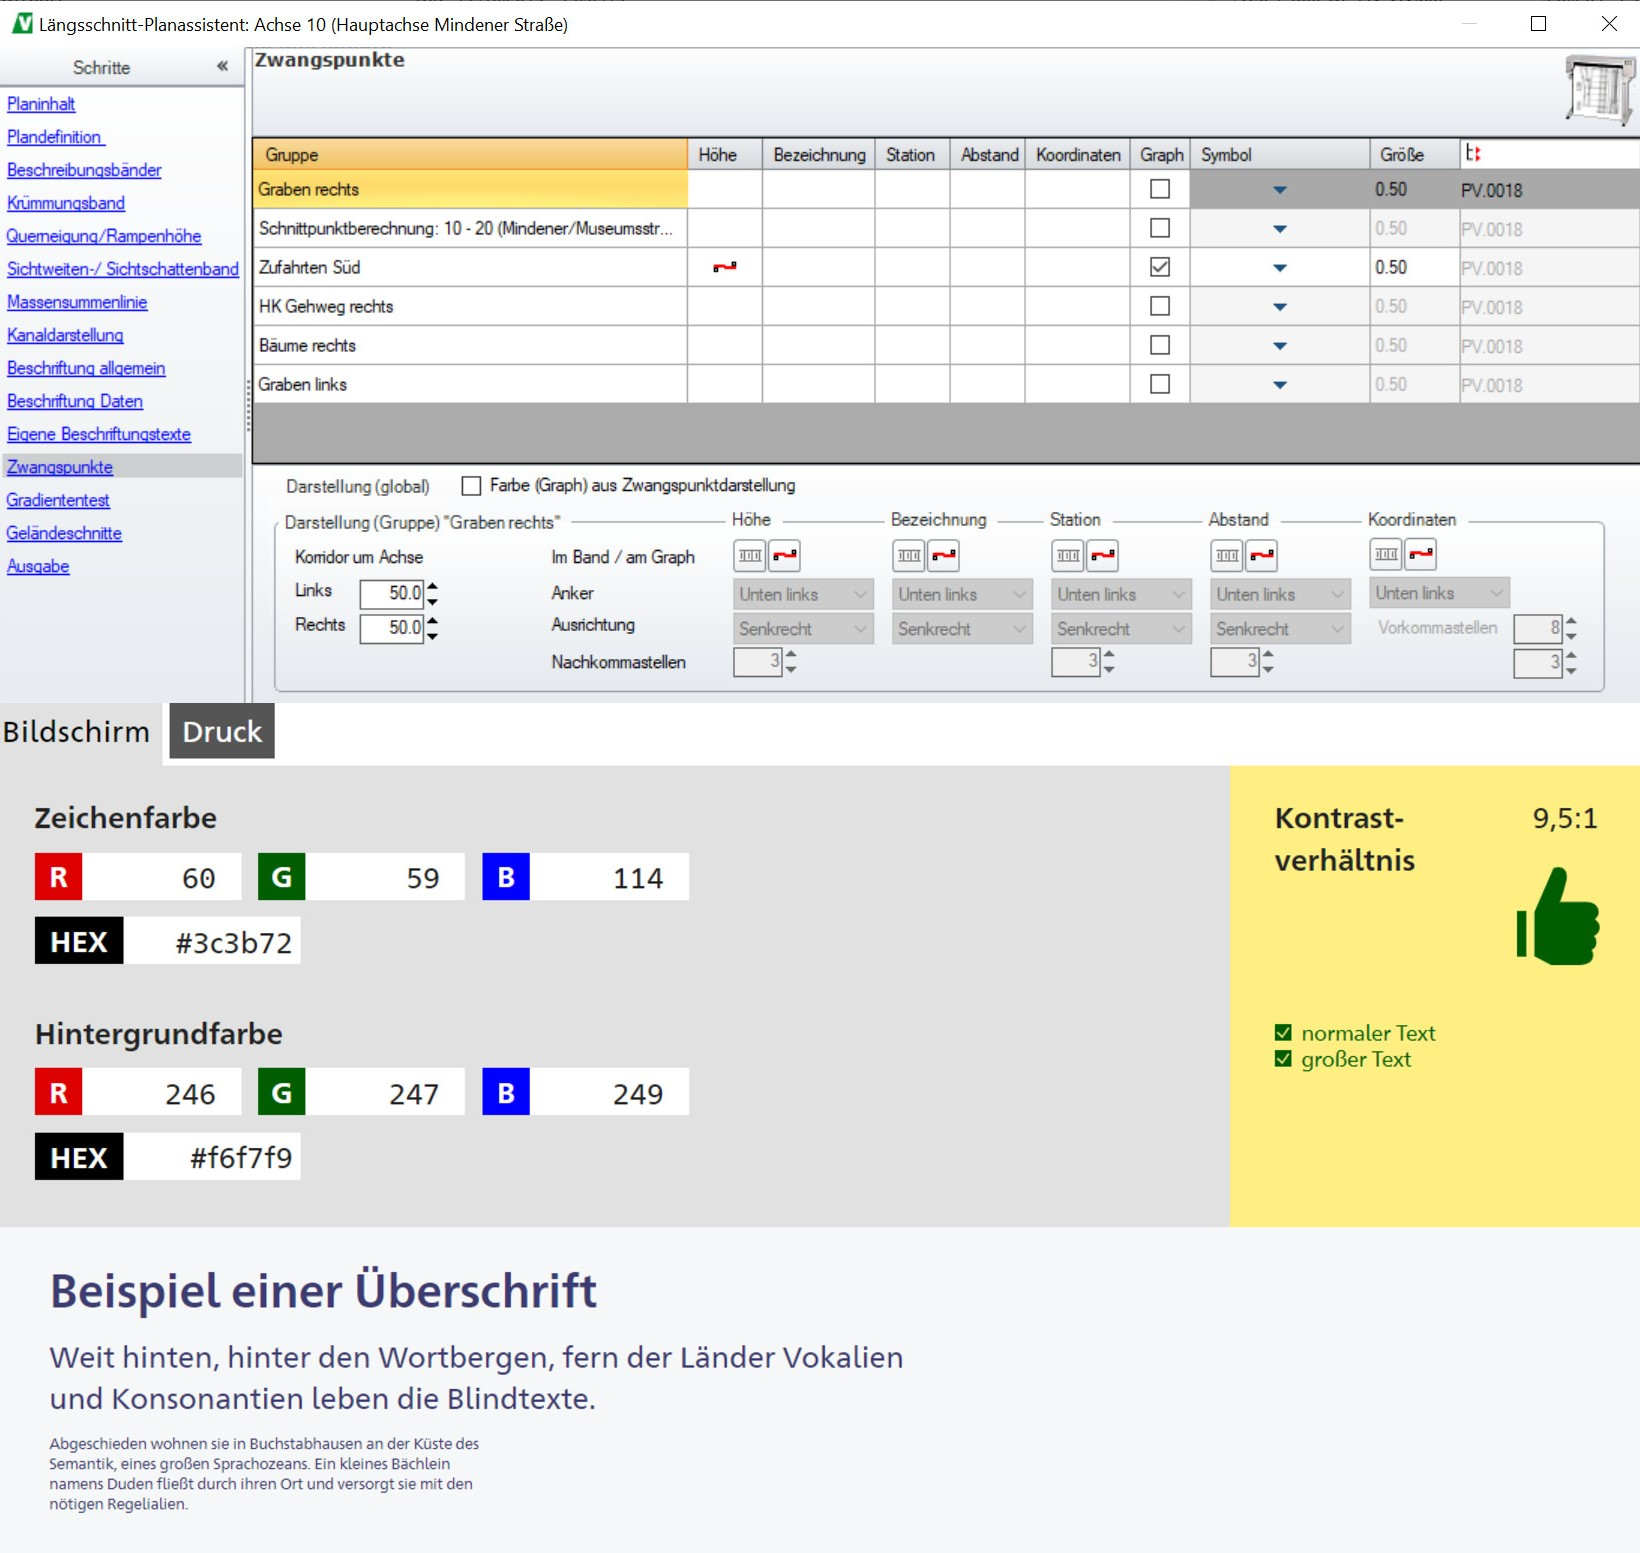
\includegraphics[width=1.0\textwidth]{Text-Kontrast}
		\caption[Text-Kontrast eines der Dialoge der Desktopsoftware]{Text-Kontrast eines der Dialoge der Desktopsoftware\\\textbf{Quelle:} Eigene Darstellung}
		\label{fig: Text-Kontrast}
	\end{figure}
	
	Wie in \cref{fig: Text-Kontrast} zu erkennen ist das Kontrastverhältnis 9,5:1, ist also sowohl für normaler Text als auch für größer Text sehr gut.
	
	\item[Tastaur-Kurzbefehle] \hfill \\
	Die \cref{fig: Kurzbefehle-Umstellen} zeigt den Dialog, wo der Benutzer die Tastatur-Kurzbefehle umstellen kann.
	
	\begin{figure}[H]
		\centering
		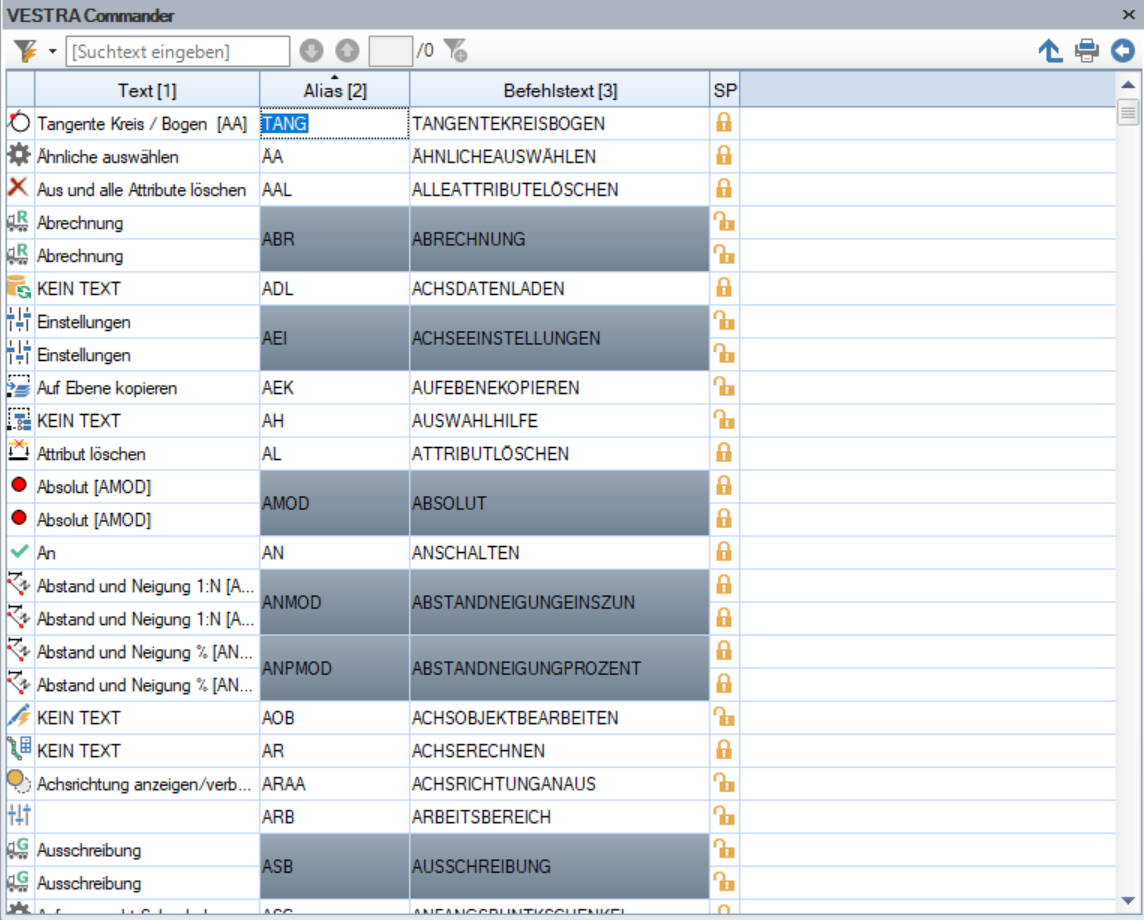
\includegraphics[width=1.0\textwidth]{Kurzbefehle-Umstellen}
		\caption[Der Dialog zur Umstellung der Tastatur-Kurzbefehle]{Der Dialog zur Umstellung der Tastatur-Kurzbefehle\\\textbf{Quelle}: Eigenes Screenshot}
		\label{fig: Kurzbefehle-Umstellen}
	\end{figure}
	
	\item[Fehlererkennung] \hfill \\
	In diesem Dialog auf der \cref{fig: Fehlererkennung} werden falsche Eingaben erkannt und dem Benutzer präsentiert (Im rechten Teil auf der \cref{fig: Fehlererkennung} wird der 
	Fehler unten im Dialog angezeigt)
	
	\begin{figure}[H]
		\centering
		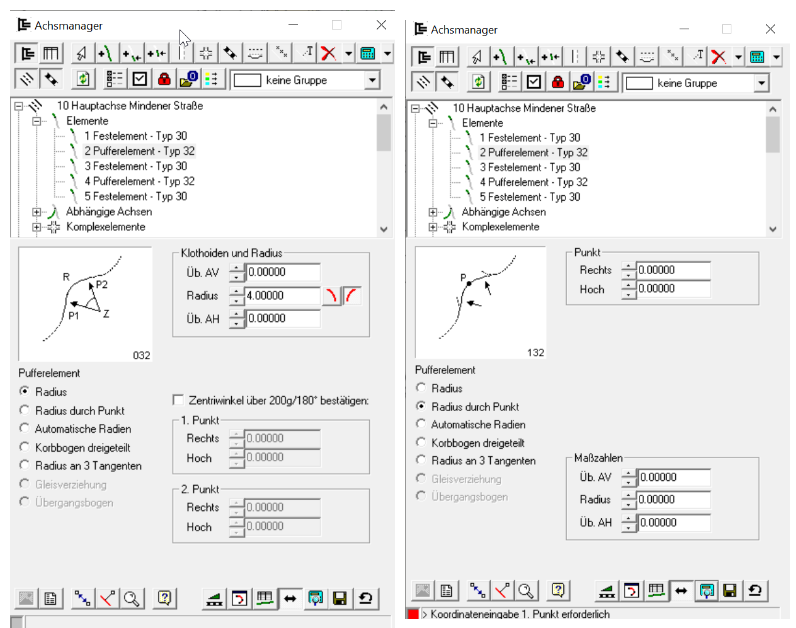
\includegraphics[width=1.0\textwidth]{Fehlererkennung}
		\caption[Fehlererkennung bei fehlerhafter Eingabe]{Fehlererkennung bei fehlerhafter Eingabe\\\textbf{Quelle}: Eigenes Screenshot}
		\label{fig: Fehlererkennung}
	\end{figure}
	
	\item[Linkzweck] \hfill \\
	Normale links werden beispielsweise von einem Screenreader Buchstabe für Buchstabe vorgelesen und damit wird der Zweck des Links niemals vermittelt. Die Hyperlinks hingegen stellen solche 
	Hindernisse nicht, da der Link implizit eingegeben ist und ein Screenreader kann ihn als normaler Text vorlesen.
	
	\begin{figure}[H]
		\centering
		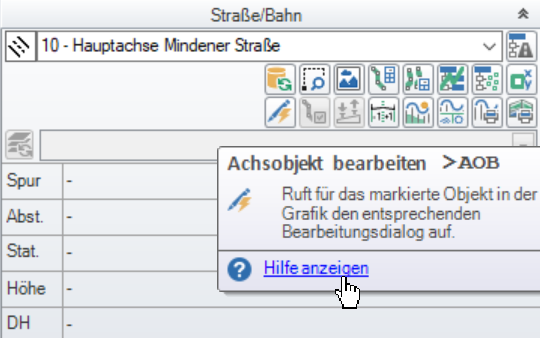
\includegraphics[width=1.0\textwidth]{Linkzweck}
		\caption[Verwendung von Hyperlink anstatt vom normalen Link]{Verwendung von Hyperlink anstatt vom normalen Link\\\textbf{Quelle}: Eigenes Screenshot}
		\label{fig: Linkzweck}
	\end{figure}
\end{description}

\vspace{2em}

\subsection*{Anlage 5}
\label{subsec: Anlage5}

\textbf{Katalog der umsetzbaren Kriterien in Dialogen der Desktopanwendungen der AKG-Software}\footnote{Eigene Darstellung}

\addcontentsline{lot}{table}{3 \hspace{1.5em} Katalog der umsetzbaren Kriterien in Dialogen der Desktopanwendungen der AKG-Software}
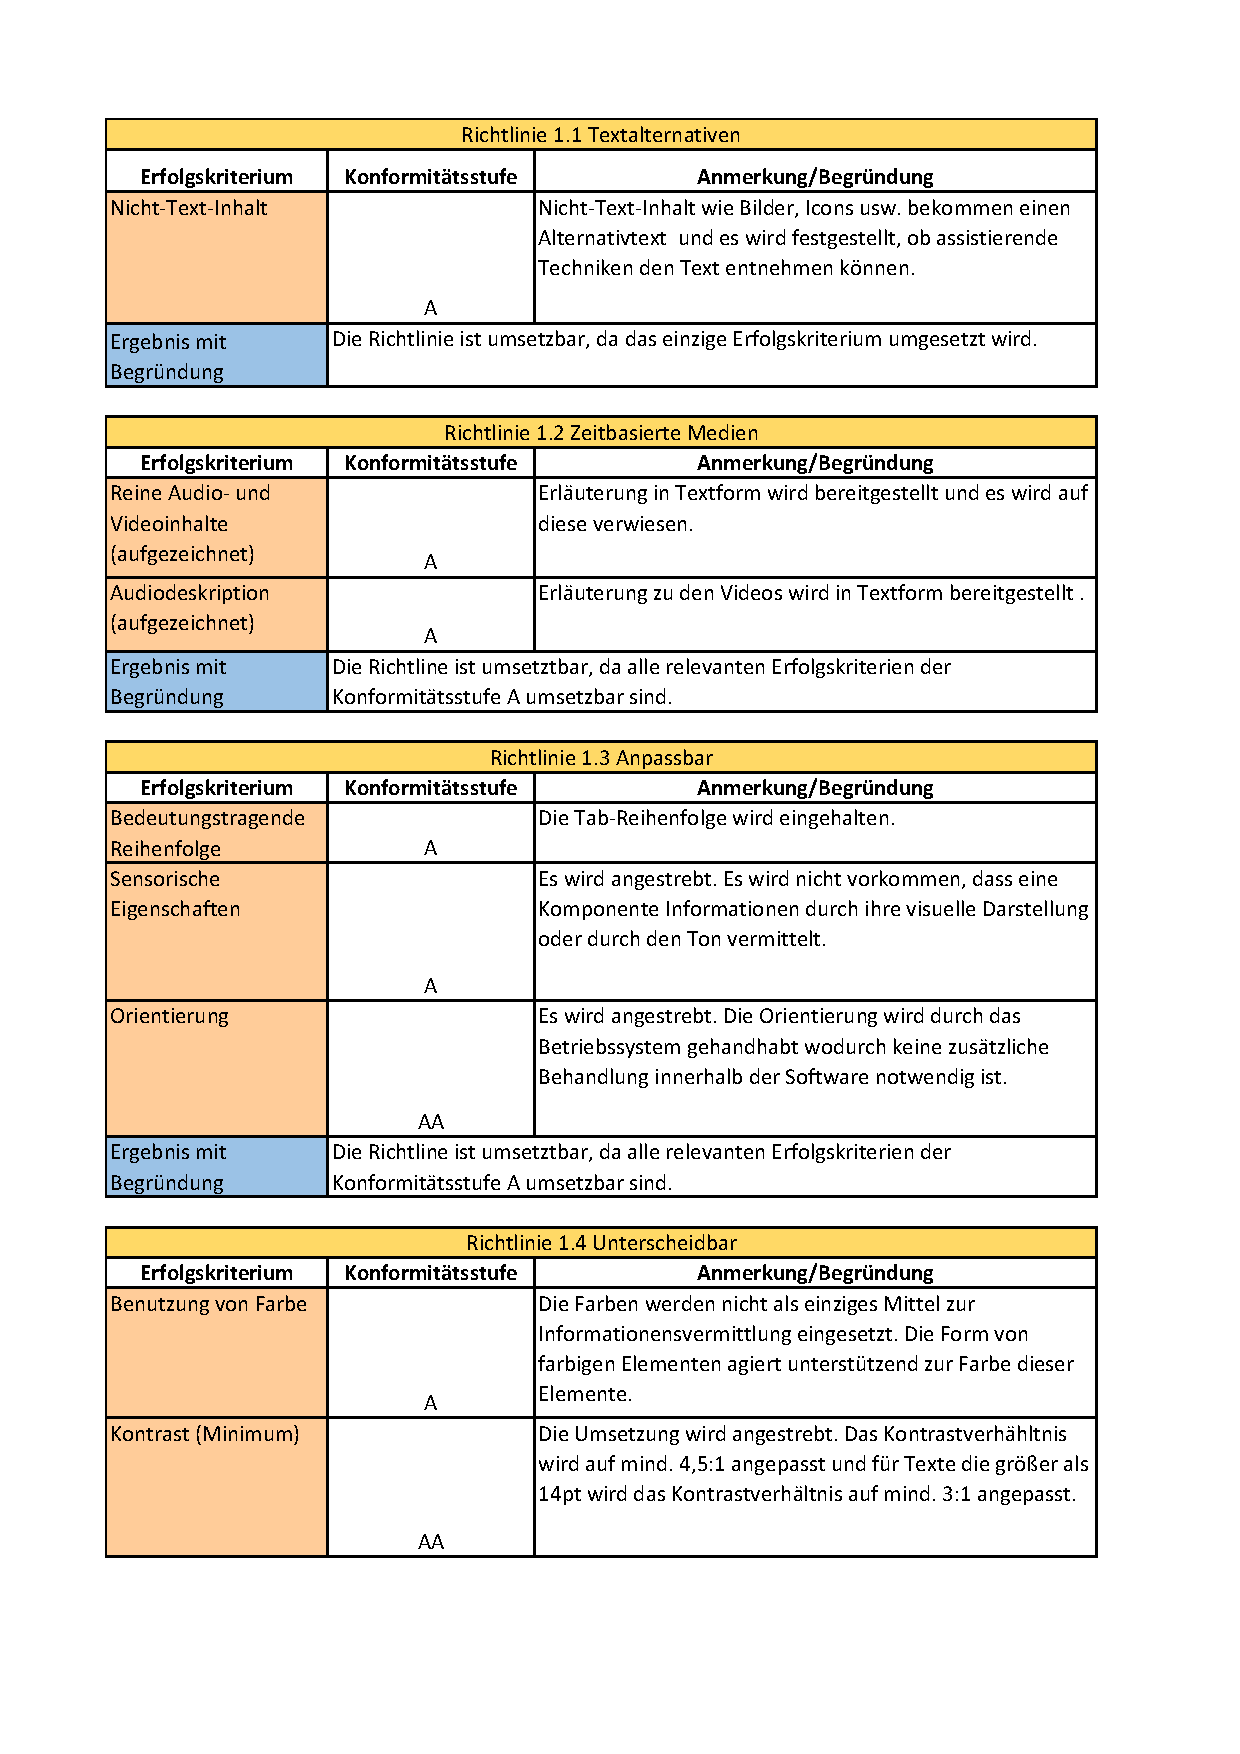
\includepdf[pages=-, scale=0.9, pagecommand={}, ]{Umsetzbare Kriterien}
